\chapter{Pipeline Shell}
\label{ch:PipelineShell}

%\textbf{\Cref{issReq:update}}
%\textbf{\Cref{issReq:maintained}}

The \gls{ps} is a shell built around an ISS, that should control the ISS, gather the resulting state changes from the ISS, and output these at the correct time. The pipeline shell should also take in the asynchronous inputs, determine when and how these should be handled, control the ISS, and adapt the output accordingly. 

\section{Implementation strategy}
\tmp{Her eller introduksjon? eller ikke i det hele tatt?}

\begin{enumerate}
    \item Implement Spike integration by stepping spike when the core retires an instruction.
    \item This should pass all synchronous tests, but not asynchronous interrupt and debug tests
    \item Make test to pass interrupts to the RM and core
    \item Pass interrupts to spike in sync with RVFI from the core to develop correct interrupt handling in spike
    \item Pass interrupts to RM asynchronously. The directed test should fail since no pipeline shell is implemented
    \item Develop pipeline shell to correctly time interrupts. The directed test should pass
    \begin{enumerate}
        \item Model simple sequential pipeline that passes synchronous tests
        \item Handle interrupts correctly in situations where interrupts can be taken immediately
        \item Correctly model each of the signals in \sv{interrupt_allowed} to properly time interrupts in instances when they can not be taken immediately
        \item Correctly move the instructions through the pipeline so the signals in \sv{interrupt_allowed} are properly timed
    \end{enumerate}
\end{enumerate}

\section{Pipeline Shell Requirements}

The following list are the requirements for the pipeline shell to correctly fit into the reference model design proposed in \Cref{ch:design}. The requirements are referred to as \textbf{PS requirement X} in the previous chapters.
In this chapter, the requirements will guide the design choices of the pipeline shell.

\begin{enumerate}

\item \textbf{RVFI from ISS.} \label[psReq]{psReq:rvfiIn}
\par The pipeline shell should use \acrshort{rvfi} as the input interface from the ISS.


\item \textbf{Take asynchronous events as inputs.} \label[psReq]{psReq:async_input}
\par The pipeline shell should take asynchronous events like interrupts and debug requests as inputs, independently of the core.

\item \textbf{Control asynchronous inputs to the ISS.} \label[psReq]{psReq:async_control}
\par The pipeline shell should control when the ISS should take an asynchronous event.

\item \textbf{Control the ISS.} \label[psReq]{psReq:ISS-control}
\par The pipeline shell should control the ISS. Including when it should execute instructions and when it should take asynchronous events.

\item \textbf{Simulate pipeline details.} \label[psReq]{psReq:pipeline}
\par The pipeline shell should simulate the necessary pipeline details to time asynchronous events. This includes stepping and flushing the pipeline.

\item \textbf{Time necessary side effects} \label[psReq]{psReq:side-effects}
\par The pipeline shell should time side effects that affect the timing of asynchronous events. 

\item \textbf{The pipeline shell should be the only core-dependent component} \label[psReq]{psReq:core-dependent}
\par 

\item \textbf{Output RVFI state at retirements} \label[psReq]{psReq:rvfiOut}
\par The pipeline shell should output RVFI to be compared with the core.


\item \textbf{Support formal verification} \label[psReq]{psReq:formal}
\par The pipeline shell should be synthesizable and support formal verification.


\end{enumerate}

\section{General architecture}

As discussed in \Cref{ch:design}, the pipeline shell should control the functional ISS, and correctly time the output state changes from the ISS. According to \Cref{psReq:rvfiIn}, the ISS should return the state changes as RVFI signals and output RVFI on retirements (\Cref{psReq:rvfiOut}).


\subsection{Pipeline Shell Design}

\Cref{sec:pw_pipelineShellDesign} describes two possible pipeline shell designs; a \textit{stage-based pipeline simulation} modeled closely to an actual pipeline, and a \textit{cycle-based time wheel simulation}, similar to the approach by \textcite{chiangEfficientTwolayeredCycleaccurate2009}. 

The cycle-based approach stores the state changes into individual stages for each cycle, while the stage-based approach operates more closely to a normal pipeline.
\Cref{sec:pw_pipelineShellDesign} highlights some disadvantages of using a cycle-based approach, as the design complicates some operations like flushing. 

When considering a pipeline shell compatible with formal verification(\Cref{psReq:formal}), even more disadvantages with a cycle-based approach are uncovered. The cycle-based approach proposed by \textcite{chiangEfficientTwolayeredCycleaccurate2009} is written in SystemC. Since the \textit{time wheel} must have one stage for every cycle that an instruction is in the pipeline, the time wheel must have a dynamic size. This is problematic because dynamic arrays in SystemVerilog are not synthesizable\cite{mehtaIntroductionSystemVerilog2021}, and therefore not compatible with formal verification\cite{seligmanFormalVerificationEssential2015}.

\textbf{Design choice:} Because of this, we choose to go with a stage-based pipeline shell. By doing so, we also have to be aware of the problem discussed in \Cref{sec:pw_pipelineShellDesign}, where bugs can be implemented the same way in both the reference model and core, and be undetected.

The architecture of the pipeline shell is shown in \Cref{fig:pipeline_shell}. This shows the four pipeline stages in the CV32E40S. We choose to use a Controller module that controls the stages. The Controller contains the most core-specific functionality, and the pipeline stages are kept relatively simple. 



\begin{figure}
    \centering
    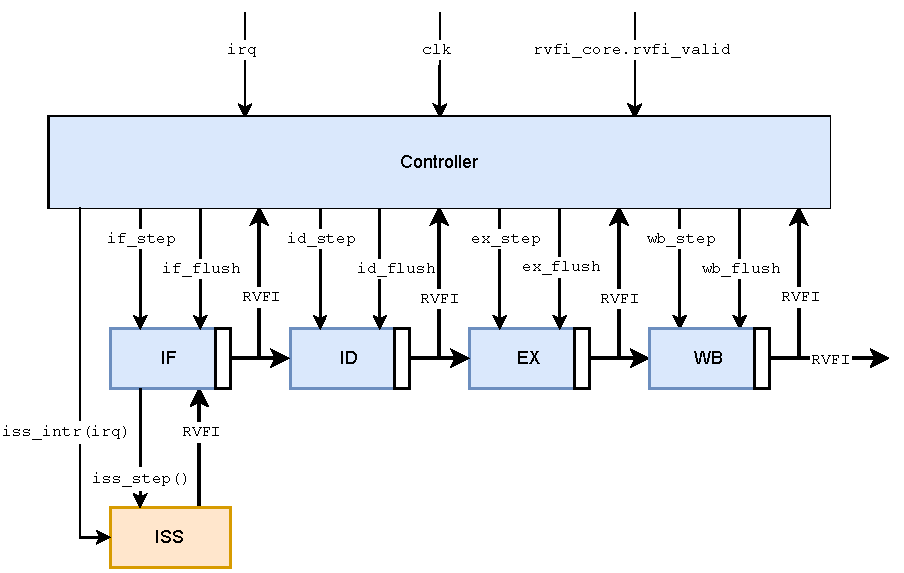
\includegraphics[width=0.75\linewidth]{figures/Pipeline_shell.pdf}
    \caption{Architecture of pipeline shell}
    \label{fig:pipeline_shell}
\end{figure}

\subsection{Interaction with the ISS}

The figure also shows that we interact with the ISS from the IF stage, where we step the ISS and get RVFI in return. This choice comes from the discussion in \Cref{sec:pw_partition}, describing how making only one call from IF to the ISS per instruction is beneficial.

Calling the ISS from the IF stage offers a key advantage: all information about an instruction's execution is available as it progresses through the pipeline, simplifying the design compared to calling the ISS from the WB stage. 

If the ISS is called from the WB stage, we do not have any information about the instructions before the WB stage. Since the controller depends on the information in the pipeline stages, decoding must happen separately from the main call to the ISS in WB. This either requires splitting up the the ISS call to separate fetching and decoding from the execution and writeback part. Additionally, branches and jumps need to be handled outside the ISS to keep the contents of the pipeline stages accurate. This would be complicated as a branch might depend on a register value, which again might require forwarding and execution to be implemented.

\textbf{Design choice:} To avoid the added complexity of calling the ISS from the WB stage, we decide to call the ISS from the IF stage. This does, however, also have multiple downsides that will be discussed later, like reversion of the ISS state on pipeline flushes (\Cref{sec:ps_revertion}) and timing of side effects in (\Cref{sec:ps_side-effects}).
%
%\subsection{Compartementalizing core-specific functionality}
%
%The pipeline shell should contain the core-specific timing implementation and be modifiable to different cores. To make it easy to configure for new cores, we should also compartmentalize the core-specific details of the pipeline shell so necessary modifications for a new core are kept to a minimum.
%


\section{Dependency of core}
\label{sec:ps_dependency}

Multiple options exist when deciding when instructions should move through the pipeline shell. We can separate these options into two categories: A \textit{retirement dependent approach}, where instructions are moved through the pipeline based on retirements from the core, and a \textit{core independent approach}, where the reference model is fully independent of the core and has to fully model the pipeline movement independent on what the core does. 

\subsection{Retirement dependent pipeline shell}

In a retirement-dependent pipeline shell, instructions are moved through the pipeline stages based on instruction retirements from the core. Each time an instruction is retired, the instructions still in the pipeline are moved one stage forward. This is similar to a \textit{step-and-compare} approach from \Cref{sec:bg_verificationTech} where the ISS steps through an instruction when an instruction retires from the core. This allows the core and reference model to easily stay in sync without exactly mirroring the cycle-accurate execution of the core.


\subsection{Core independent pipeline shell}

In a core-independent pipeline shell, the execution would be fully independent of the core, and the movement of instructions through the pipeline would be completely contained in the pipeline shell. This complicates the pipeline shell because the pipeline shell has to mirror the exact execution of the core at every cycle. It must account for forwarding hazards and stalls, the exact cycle delay for \acrshort{lsu} operations, the exact cycle count of multi-cycle instructions, etc.

Instructions can be moved through the pipeline mirroring the functionality of the core, where every clock each stage reports if it is ready to receive new data, and if each stage has valid data ready, and uses this to move the data through the pipeline. Additionally, there are signals for pending interrupts, jumps, branches, exceptions, multi-cycle instructions in progress, etc. that must be considered. 

The CV32E40S user manual contains a table with the number of clock cycles for every multi-cycle instruction \cite{openhwgroupPipelineDetailsCOREV2023}. If we do not rely on the retirement from the core, we must use this table to determine how long an instruction should take in each stage. This can be complicated as we need to have specific cases for every instruction, and some instruction types have different clock cycles for different situations.

%\tmp{40s security feature}

\subsection{comparison}

\begin{table}[htb]
\centering
\caption{Comparison of retirement and clock driven pipeline}
\label{tab:retirementvsclock}
\begin{tabularx}{\textwidth}{|p{15mm}|*{2}{>{\arraybackslash} X |}}
\hline
 & Advantages & Disadvantages \\
\hline
Retirement dependent
& \begin{itemize}
\item Simpler to model
\item Lower chance of implementing bugs from the core
\end{itemize}
& \begin{itemize}
\item Does not test if instructions retire after the right amount of cycles (Not that important?)
\item Add specific stall cases instead of movement cases
\item Will not be equal at every clock cycle
\item 
\end{itemize} \\
\hline
Core independent
& \begin{itemize}
\item Cycle-accurate equal to core
\item Can be used to verify that the core uses the correct amount of cycles for each instruction. 
\end{itemize}
& \begin{itemize}
\item Hard to implement. Essentially all timing-related implementations must be implemented in the core
\item We must calculate the cycle count for all instructions and edge cases.
\end{itemize} \\
\hline
\end{tabularx}
\end{table}

As discussed in \Cref{sec:des_retireOrClock}, we will only compare the state after each retirement, but cycle-accurate detail influences this as explained in \ref{}\tmp{TODO}.
Since we only compare the core and reference model at instruction retirements, it might be sufficient with a retirement-dependent pipeline shell. If this works, it would be easier to implement and less complicated. We would not need to model as much of the core-specific details. To avoid the possibility of implementing the same bugs that might be in the core, we want to avoid implementing detailed core-specific details as much as possible.

\textbf{Design choice:} We will focus on a retirement-dependent pipeline shell going forward to determine if this is sufficient. 



%\begin{enumerate}
%    \item Should the pipeline shell calculate the correct clock cycle for each instruction? Hard for division etc which is variable.
%    \item Can retirements be used and potential "bubbles" be calculated instead of all details 
%    \item What in the dependency graph can be wrong if we only move the pipeline on retirements?
%    \item - Can these occurrences be specifically handled, instead of accurately calculating all "instruction movements?"
%    \item How should stalls be calculated?
%    \item How should pipeline flushes be handled?
%    \item How should multi cycle instruction be handled?
%\end{enumerate}


\section{Pipeline stage modeling : \Cref{psReq:rvfiIn}, \ref{psReq:pipeline}, \& \ref{psReq:rvfiOut}}

This section will cover the design choices for the pipeline stages in the pipeline shell. 

\subsection{pipeline stage register content}

From \Cref{psReq:rvfiIn}, the ISS returns an RVFI struct after it executes an instruction. To avoid storing the full RVFI interface, only the essential variables are sent from the ISS through the \sv{st_rvfi} struct. We also want to store this struct in the pipeline shell.  We combine this struct with a valid signal into the \sv{pipe_stage_t} struct passed through the pipeline. The valid signal is high when the instruction executes correctly in the ISS and goes low before the pipeline is filled up, when the pipeline is flushed, and in other situations where the instructions in the pipeline are not valid. We combine this valid signal with the step signa when the core is in the WB stage, to only mark each instruction as valid one time out of the pipeline shell.

\begin{systemverilog}
typedef struct packed {
    st_rvfi rvfi;
    logic valid;
} pipe_stage_t; 
\end{systemverilog}


%Since we use instruction retirements from the core to move through the pipeline stages, we also need to use this to output RVFI. To make sure each instruction is only marked as valid for one cycle when outputting rvfi, we need to combine the valid signal from the core, with the valid signal from the pipeline shell. This allows the RVFI output to be in sync with the core, while also only outputting RVFI when the instruction in the pipeline shell is actually valid.

%To add signals like \lstinline{rvfi_valid} we create a new interface called \lstinline{rvfi_if_t} that is passed from the pipeline shell to the reference model wrapper. 


%The WB stage therefore looks like this.
%\begin{systemverilog}
%always_ff @(posedge clk) begin
%    if (flush_i) begin
%        pipe_o.rvfi <= '0;
%        pipe_o.valid <= 1'b0;
%    end else if(step) begin
%        pipe_o.rvfi <= pipe_i.rvfi;
%        pipe_o.valid <= pipe_i.valid;
%    end
%    else begin
%        pipe_o.rvfi <= pipe_o.rvfi;
%        pipe_o.valid <= 1'b0; //Only output valid at first valid clock cycle
%    end
%end
%\end{systemverilog}



\subsection{Pipeline stages}

We want most of the timing details to happen in the controller module with our chosen architecture, leaving the pipeline modules fairly simple. This gives us the choice of making separate modules for each pipeline stage, or reusing the same module for all the stages. Although the pipeline stages should operate fairly similarly, there are some differences. For example, the IF stage must step the ISS and take in the RVFI from the ISS as an input. By making separate modules for each pipeline stage, we can specifically modify IF to call the step function, and take the RVFI result from the pipeline. If we instead use a generic stage module, we have to call the step function outside of the IF stage. 

Different cores can have different numbers of pipeline stages, so it should also be trivial to add or remove pipeline stages when configuring the pipeline shell for a new core. The pipeline shell could use a generate construct to change the number of pipeline stages. This would also lead to a differing number of inputs and outputs to the controller module, which should control each step. For this, an interface could be used with a configurable number of control signals for each pipeline stage. Alternatively, we can have different pipeline shell files for each core in separate directories that can be more specialized for the core. A parameterizable amount of pipeline stages could work for in-order pipelines, but this could get more complicated if we also consider out-of-order pipelines. This report will focus on in-order pipelines, but to possibly also allow out-of-order pipelines, we choose to go with the second option, where all the pipeline shell files are specific to a core.

%\tmp{TODO: Use an interface with rvfi and control signals instead of individual signals.}

%\textbf{Design choice:} Use a generic pipeline stage module, or specific for each stage? \tmp{currently specific but not justified}
%
%Generic: easier to add more pipeline stages.
%
%Specific: Not all pipeline stages are equal.
%
%For the IF stage, we call the \sv{iss_step()}function to step spike. This can either be done inside of the if module with a specific stage module, or outside the module and passed in as a \sv{pipe_stage_t} input, that is used by the other stages to move data from the previous stage.
%
%\tmp{The core has a delay between the WB stage and the RVFI output, replicate this in the RM or use straight out of WB?}
%
%
%\tmp{General or specific pipeline stage modules? IF and WB are slightly different compared to the others.}


%\subsection{Register in the WB stage}
%
%As shown in \Cref{fig:cv32e40s-block}, the CV32E40S core the pipeline has 3 registers between the 4 pipeline stages: \sv{IF_ID},\sv{ID_EX}, and \sv{EX_WB}. What is not shown in the figure is that the RVFI output, which should be valid when an instruction is retired, is actually delayed one cycle from when the instruction reaches the WB stage. To simulate this behaviour in our pipeline shell, we also add a register after the WB stage, giving us the pipeline in \Cref{fig:pipeline_shell}

\section{Controller module design}

The controller is the module that actually controls the movement of the pipeline stages, and is the part of the reference module that contains the most core-specific functionality. It takes in most of the inputs to the pipelines shell, as well as the state from each pipeline stage. It should be responsible for using the inputs for the following tasks, which will be discussed in the sections:

\begin{enumerate}
    \item Determine when to step the ISS and pipeline stages based on retirements from the core
    \item Determine when to take asynchronous events such as interrupts, debug requests, and \acrshort{nmi}s
    \item Control flushing of the pipeline stages and reversion of the ISS state
\end{enumerate}

%\subsubsection{Input signals}
%\begin{itemize}
%    \item \sv{clk}
%    \item \sv{rst}
%    \item \sv{valid} (Retirement from the core)
%    \item \sv{irq_i} 
%    \item \sv{if_id_pipe_i}
%    \item \sv{id_ex_pipe_i}
%    \item \sv{ex_wb_pipe_i} 
%    \item \sv{wb_pipe_i}
%    \item \sv{interrupt_allowed_i} interrupt allowed from the core
%    \item \sv{mstatus.mie} from the ISS
%\end{itemize}
%
%\subsubsection{Output signals}
%\begin{itemize}
%    \item \sv{\{if,id,ex,wb\}_step_o}
%    \item \sv{\{if,id,ex,wb\}_flush_o}
%    \item \sv{interrupt_allowed_o}
%\end{itemize}

\section{Instruction stepping : \Cref{psReq:ISS-control}}

We will use the word \textit{\gls{step}} to mean when the ISS executes one instruction and when an instruction moves from one pipeline stage to another. When implementing a retirement-dependent pipeline shell, we want to step the ISS and pipeline stages when the core retires an instruction.

In a normal pipeline, the movement of instructions in the pipeline is controlled by a \sv{ready} and a \sv{valid} signal in each pipeline stage. When both the previous stage has \sv{valid} data, and the next stage is \sv{ready} to receive new data, the instruction data is moved into the next pipeline register.

Since we use a step function in the ISS and a simplified pipeline, we can instead use a \sv{step} signal to step the pipeline. The same step signal can be used to step the ISS and the pipeline to ensure this happens in sync.

To step the ISS, we need a function that will step one instruction when called. This gives us \textbf{\Cref{issReq:step}}. Since we use a retirement-dependent approach, we will call this step function when the core retires an instruction and the \sv{rvfi_valid} signal is high. 

\subsection{halting}

In a normal pipeline, every stage can be halted, where the pipeline stage will not be valid or ready, meaning it will not be updated with a previous instruction or output its value to a new stage. Since we use a \sv{step} signal to signal when an instruction should step into the next pipeline stage or not, this implicitly supports halts without needing a separate halt signal. 

\subsection{Filling the pipeline}

At the very beginning of a simulation and after the pipeline is flushed, it contains multiple empty stages. If we wait for the first retirement from the core before executing any instructions in the reference model, it would be delayed behind the core since it takes multiple steps to fill up the pipeline and output instructions. 

Because of this, we want to fill up the pipeline when it is not full so that the next retirement from the core also triggers a retirement from the reference model.

To implement this functionality, we use a \sv{pipe_count} counter that starts at 0 at the beginning and is reset to 0 during a full pipeline flush. This counts up to the number of pipeline stages every time a step is done. This keeps track of how many instructions are in the pipeline. When the counter is lower than the number of pipeline stages, we set \sv{step} high so the pipeline can fill up. When the pipeline is filled, the \sv{step} signal is controlled by the \sv{rvfi_valid} signal from the core. 
%\begin{systemverilog}[label={lst:pipe_count}, caption={Systemverilog code for filling the pipeline at the start and after a flush.}]
%
%assign pipeline_full = pipe_count >= (PIPELINE_DEPTH - 1);
%
%// Count the amount of filled pipeline stages at the start or after a flush 
%always_ff @(posedge clk) begin
%    if (rst_n == 1'b0 || flush_pipeline)begin 
%        pipe_count <= 0;
%    end else if (!pipeline_full) begin
%        pipe_count <= pipe_count + 1;
%    end else begin
%        pipe_count <= pipe_count;
%    end
%end
%// step the pipeline until the first stages are filled up to be in sync with the core
%always_comb begin
%    if (rst_n == 1'b0) begin
%        step <= 1'b0;
%    end else if (!pipeline_full) begin
%        step <= 1'b1;
%    end
%    else if (valid) begin
%        step <= 1'b1;
%    end
%    else begin
%        step <= 1'b0;
%    end
%end
%\end{systemverilog}




\section{Interrupt : \Cref{psReq:ISS-control}}
\label{sec:ps_interrupt}

This section will cover how interrupts are taken in the pipeline shell. This includes partitioning interrupt handling between the ISS and pipeline shell and how the interrupt is handled in the pipeline shell.  

\subsection{Partitioning of interrupt handling between the ISS and pipeline shell}

We must decide whether to take an interrupt in the pipeline shell or in the ISS. We can split this decision into when and which interrupt should be taken.

\subsubsection{Decision in pipeline shell or ISS}

\tmp{Er det greit her, eller burde dette være ie Chapter 4?}

From \Cref{fig:interrupt_timing}, we see that deciding on taking an interrupt depends on \sv{pending_interrupt} and \sv{interrupt_allowed}. \sv{pending_interrupt} depends on the incoming interrupt and values from the CSR, while \sv{interrupt_allowed} depends on the content of the pipeline. We will consider these separately.

Since only \sv{interrupt_allowed} depends on the pipeline content, while only \sv{pending_interrupt} depends on the CSR, we can split these between the pipeline shell and the ISS.

The pipeline shell of the reference model does not have access to all the CSRs without exporting them from the \acrshort{iss}. To determine the \sv{pending_interrupt} signal to decide if the incoming interrupt is enabled, it needs to know the values of \sv{mie}, \sv{mstatus.mie}, the privilege level, and debug mode \cite{openhwgroupCv32e40s2024}. As these are all kept inside the \acrshort{iss}, we either have to export these from the ISS or determine if the interrupt will be taken inside the ISS. 

The \sv{interrupt_allowed} signal depends on the pipeline content of the pipeline shell, making it more logical to implement in the pipeline shell than the ISS.


\tmp{PGK: Dette valget har vist seg å ikke være det beste. Hvor bør jeg diskutere dette?}
\textbf{Design choice:} The ISS should decide the \sv{pending_interrupt} part of taking an interrupt, while the pipeline shell should decide if the interrupt is allowed with \sv{interrupt_allowed}.

Implementing the \sv{interrupt_allowed} signal in the pipeline shell will be covered further in \Cref{sec:interrupt_allowed}.

\subsubsection{Which interrupt to take}

We can either determine which interrupt to take in the pipeline shell or in the ISS. Deciding this in the ISS simplifies the interface to the ISS, since we can inject the whole \rv{irq} register into the ISS as is, to be set in the \rv{mip} register. 

By accurately setting the \rv{mip} bits in the ISS, we would assume that it should be able to determine which interrupt to take given the RISC-V Specification.
This is not actually the case. The RISC-V specification only specifies the correct order of the standard interrupts specified in bit 15:0 in \rv{mip}, but not for the custom interrupt bits at bit 16 and above \cite{watermanRISCVInstructionSet2021}. If the ISS should decide the order of interrupts, some platform or core-specific interrupt handling information must be implemented in the ISS.

On the other hand, determining the interrupt ordering in the pipeline shell causes some problems with the communication with the ISS. Instead of injecting the bits to be set in \rv{mip} and letting the ISS operate close to its original implementation, larger modifications to interrupt handling are required. If we want to tell the ISS which interrupt to take, the ISS must be modified to take the input interrupt instead of analyzing \rv{mip} and deciding the interrupt. One approach to informing the ISS of the interrupt is to only set one \rv{mip} bit at a time, so the ISS has no choice. This can work, but causes a mismatch between the \rv{mip} register of the core and the reference model if this is read. Another way would be to override the ISS interrupt-taking functionality so that it takes a given input interrupt instead of relying on \rv{mip}.

\textbf{Design choice:} We choose to let the ISS decide which interrupt to take, given the incoming \rv{mip} bits. This requires that the interrupt priority in the ISS is configured the same way as the core, giving us \textbf{\Cref{issReq:interruptOrdering}}.

\subsection{Interrupt notification to the ISS}

To inform the ISS of interrupts, we use a dedicated function called \sv{iss_intr()}. This is called every clock cycle and takes \sv{irq} and \sv{interrupt_enabled} as inputs.

We choose a separate function instead of using the \sv{iss_step()} function since we only run \sv{iss_step()} on instruction retirements, and we want to notify the ISS if interrupts independently of retirements since the ISS decides if the interrupt should be taken or not.

The \sv{iss_intr()} function updates the \rv{mip} bits based on the incoming \rv{irq} and the bits set in the \rv{mie} CSR. If the \sv{interrupt_enabled} signal is high, the ISS should choose whether to take the interrupt and return a boolean value indicating its decision. If interrupts are not enabled, it should still set the \rv{mip} bits, but the interrupt should not be taken. This requires that the ISS can enable or disable interrupts independently of the \rv{mip} bits and other CSRs. This gives us \Cref{issReq:interruptEnabled}. 



\subsection{Interrupt allowed}
\label{sec:interrupt_allowed}

\tmp{Hvordan funkerer denne seksjonen? Bør jeg ha med (og rydde i) LSU interruptible eksempelet?, eller snakke mer generelt om interrupt allowed}

The \sv{interrupt_enabled} signal in the CV32E40S core determines whether an interrupt can be taken based on the current pipeline state. The signal is influenced by various factors, including the status of in-flight memory operations, debug mode restrictions, ongoing multi-cycle instructions, and other pipeline-related conditions. \Cref{fig:dependency-tree-cv32x} shows the complexity of this signal and how it depends on the different pipeline stages.


All components contributing to the \sv{interrupt_allowed} signal would ideally be accurately modeled to create a reference model independent of the core. The content of each pipeline stage in the pipeline shell should be used in order to model the \sv{interrupt_allowed} signal independently of the core. 

However, due to the scope of this thesis, the \sv{interrupt_allowed} signal is not modeled based on the pipeline shell, but Instead directly injected from the DUT core. This is done to facilitate the implementation of the other reference model components, where we can assume that the \sv{interrupt_allowed} signal functions correctly.

Both when injecting the \sv{interupt_allowed} signal from the core and when recreating the signal, we have the possibility of modeling the same bugs as the core. If there is a bug in the implementation of this signal in the core, we could end up modeling the same bug in the reference model, and the bug would not be detected. For example, if the core incorrectly allows an interrupt to be taken when there is an outstanding memory operation, the reference model could also allow the interrupt to be taken, and there would be no mismatch between the core and reference model.

This reliance on the \sv{interrupt_allowed} signal is one considerate disadvantage of this implementation. It is important to be mindful of this limitation and avoid using the implementation from the core as much as possible when implementing this in the reference model.

%\subsection{Example: LSU interruptible Signal}
%\tmp{PGK: Har bare sett litt på LSU interruptible, men ikke de andre komponentene til interrupt allowed. Bør jeg ha med dette som ett eksempel, eller er det ryddigere å ikke nevne noe mer siden jeg ikke implementerer interrupt allowed?}
%
%\tmp{TODO: Renskriv eller fjern?}
%
%The \sv{lsu_interruptible} signal is controlled by the \acrshort{lsu} in the core. It goes low when the transition has been valid for at least one clock cycle or har outstanding requests. It is reset when the transaction is done. 
%
%The amount of outstanding transfer requests is signaled by a counter \sv{cnt_q}, that counts up when a transfer request is accepted, and counts down when the transfer is done with \sv{resp_valid}.
%
%To simulate this in the reference model, we have a few considerations. We have to time when a memory request is issued, and when the response is valid.
%
%\textbf{approach 1:}
%\sv{lsu_interruptible} can be set low one cycle after a load/store instruction arrives in the EX stage.
%\sv{lsu_interruptible} can be set high again when the load/store instruction retires from the WB stage.
%
%\textbf{approach 2:}
%\sv{lsu_interruptible} can be set low one cycle after a load/store instruction arrives in the EX stage.
%The amount of clock cycles can be calculated given the instruction. Load/store instructions are handled in 1 bus transaction, while misaligned word transfers and halfword transforms use two bus transactions with two cycles in EX and 2 in WB \cite{openhwgroupPipelineDetailsCOREV2023}. This can potentially be used to calculate how long \sv{lsu_interruptible} should be low.
%
%\textbf{approach 3:}
%A uvm agent listening to OBI transactions can be used to time requests and responses to correctly simulate the \sv{lsu_interruptible} signal. This is less independent of the core execution since the timing of requests is done from the core. To avoid being dependent on the core, we can use the OBI agent to only listen for responses, but start the requests from the reference model.
%
%
%\subsubsection{experiment:}
%Will the timing of LSU requests be correct in approaches 1 and 2 by setting \sv{lsu_interruptible} low one cycle after a load/store instruction arrives in the EX stage?
%
%\subsubsection{Implementation Approach 1}
%
%To correctly time LSU requests, LSU instructions must be identified in the EX stage. To achieve this, the RVFI signals received from the ISS must be used to decide whether the instruction is a valid LSU instruction. We can either add a special signal dedicated to this or use the existing RVFI signals. To keep the RVFI interface as close as possible to the standard, it is beneficial to use the signals as they are. 
%
%
%Instead of analyzing the instruction to check if it has a memory operation, check if the memory operation is valid, etc. We can let the ISS do the work, and utilize the RVFI signals to see if a memory operation was done in the ISS. RVFI has multiple memory signals that can be used. The masks \sv{rvfi_mem_rmask} and \sv{rvfi_mem_wmask} are non-zero for read and write operations respectively. We can use these signals to determine if there is a read or write operation in the EX stage.
%
%From the specification in \Cref{lst:lsu_interruptible_spec} we see that the \sv{lsu_interruptible} signal should go low one cycle after a memory request is passed to the LSU in the EX stage, and it should go high again when a memory response is received in the WB stage. 
%
%
%\tmp{TODO}






%One disadvantage of this approach is that it leads to many more DPI function calls to the ISS, which can decrease performance.

%%\textbf{\Cref{issReq:interrupt}}.



%To signal to the ISS when an interrupt should be taken, one way is to use the \rv{mip} bits to signal when it should be taken, and set these bits to 0 when the interrupt can not be take. This is problematic because situations can occur where the \rv{irq} bits change while interrupts are not allowed. This would lead to a mismatch between the \rv{mip} bits of the core and reference model. This could mostly go unnoticed, but be problematic if a CSR read is done on the \rv{mip} bits.  





%In spike this functionality is not possible. If \sv{mip} is set, and the interrupt is enabled through the CSRs, the interrupt will be taken the next time spike steps. It is therefore not possible to disable an interrupt with \sv{interrupt_allowed} while keeping all the CSRs identical to the core. To implement the \sv{interrupt_allowed} functionality, we must either only set the \sv{mip} bits when \sv{interrupt_allowed == 1}, disable the interrupt via a CSR like \sv{mstatus.mie}, or internally modify spike to implement an additional check on a new \sv{interrupt_allowed} variable before taking an interrupt, for example modifying \ccode{void processor_t::take_interrupt(reg_t pending_interrupts)} from \file{processor.cc} \cite{SpikeRISCVISA2023}. 



%\subsection{Interupt taking}
%
%To signal to the pipeline when an interrupt is taken, and the pipeline needs to be flushed, we can either use the return of \sv{iss_intr()} that says when the interrupt should be taken or use the RVFI output from the ISS. The RVFI is only output when the core retires an instruction, but there can be some time between when the interrupt is applied and when the core retires an instruction. The \sv{interrupt_taken} signal from \sv{iss_intr()} signals when the interrupt can be taken the clock after the interrupt is signaled, more closely resembling the core functionality. 
%

%\subsection{Timing irq}
%
%\tmp{We need a 2 cycle delay between when the irq changes}
%\tmp{Because the RM is one cycle after the core, and the irq is also clocked one cycle into \sv{irq_q} in the core}







%\section{Taking an interrupt}
%
%\tmp{Use ISS to determine if it can be taken?}
%
% In the core, an interrupt is taken if both \sv{pending_interrupt} and \sv{interrupt_allowed} is true. \sv{interrupt_allowed} is explained in \Cref{sec:interrupttiming}. \sv{pending_interrupt} is high if an interrupt is set on \sv{irq_q} and the same bit is enabled in the \sv{mie} \acrshort{csr}. Additionally, the \sv{mstatus.mie} global interrupt enable \acrshort{csr} must be set, and the privilege level muse be below 
%
%By expanding the signals responsible for \sv{pending interrupt}, we get the expression in \Cref{lst:pending_interrupt}
%
%\begin{systemverilog}[label={lst:pending_interrupt}, caption={Signal requirements for \sv{pending_interrupt}}]
%    pending_interrupt = 
%    irq_req_ctrl_o = (|irq_local_qual) && global_irq_enable = 
%    (|irq_local_qual) && (mstatis_i.mie || (priv_lvl_i < PRIV_LVL_M) = 
%    (|(irq_q & mie_i)) && (mstatis_i.mie || (priv_lvl_i < PRIV_LVL_M)
%\end{systemverilog}
%
%When \sv{pending_interrupt} is high, we know that the interrupt on \sv{irq_q} will actually be taken if \sv{interrupt_allowed} also is high. 
%
%
%\subsubsection{Scenario: Set mip while \sv{interrupt_allowed = 1} and interrupt enabled.}
%
%Interrupt should be taken immediately.
%
%\subsubsection{Scenario: Set mip  while \sv{interrupt_allowed = 0}, interrupt enabled. Then set \sv{interrupt_allowed = 1}}
%
%Interrupt should be taken when \sv{interrupt_allowed} goes to 1. mip should remain set while \sv{interrupt_allowed} is 0
%
%\subsubsection{Scenario: Set mip  while \sv{interrupt_allowed = 1} and mie disabled, then later enable mie }
%
%\subsubsection{Scenario: Set mip  while \sv{interrupt_allowed = 0} and mie disabled, then later enabled enable mie, and set \sv{interrupt_allowed = 1}}
%
%
%
%\subsubsection{requirements}
%
%\sv{mip} should remain set or not while \sv{irq_q}
%In the core \sv{mip} directly follows \sv{irq_q}, independently of the other signals. 
%
%
%%In order to minimize modifications to the internal Spike code, and minimize the effect on other parts of the code, we choose to only set the \sv{mip} bits only when \sv{interrupt_allowed == 1}. 
%
%%This check can either be done in the \sv{iss_intr()} function, or before calling the function. To support the possibility changing to a solution where \sv{mip} is set independently of \sv{interrupt_allowed} like above, we implement the \sv{interrupt_allowed} check inside \sv{iss_intr()} to allow the rest of the code to be unchanged in both implementations.
%
%
%Regarding when to call the \sv{iss_intr()} function, the simplest implementation might be to call it at every positive clock edge. This avoids extra checks outside \sv{iss_intr()} to determine when it can and should be called, but instead keeps these check inside the function, dependent on implementation. 
%





\section{Timing Side effects : \Cref{psReq:side-effects}}
\label{sec:ps_side-effects}

\subsection{Side effects influencing interrupt timing}

Some side effects affect the timing of interrupts. Two examples are \rv{mstatus.mie} and \rv{mie}. To properly time interrupts, we want to apply the changes in these CSRs when they leave the WB stage in the pipeline shell, instead of when the instruction steps in the IF stage.


Since we step the instruction in the ISS in the IF stage, there are some cycles before the instruction is retired from the reference model, because it travels through the pipeline stages. If we use the CSR registers local to the ISS, these might not be the same as if they were updated in the WB stage.

\begin{figure}
    \centering
    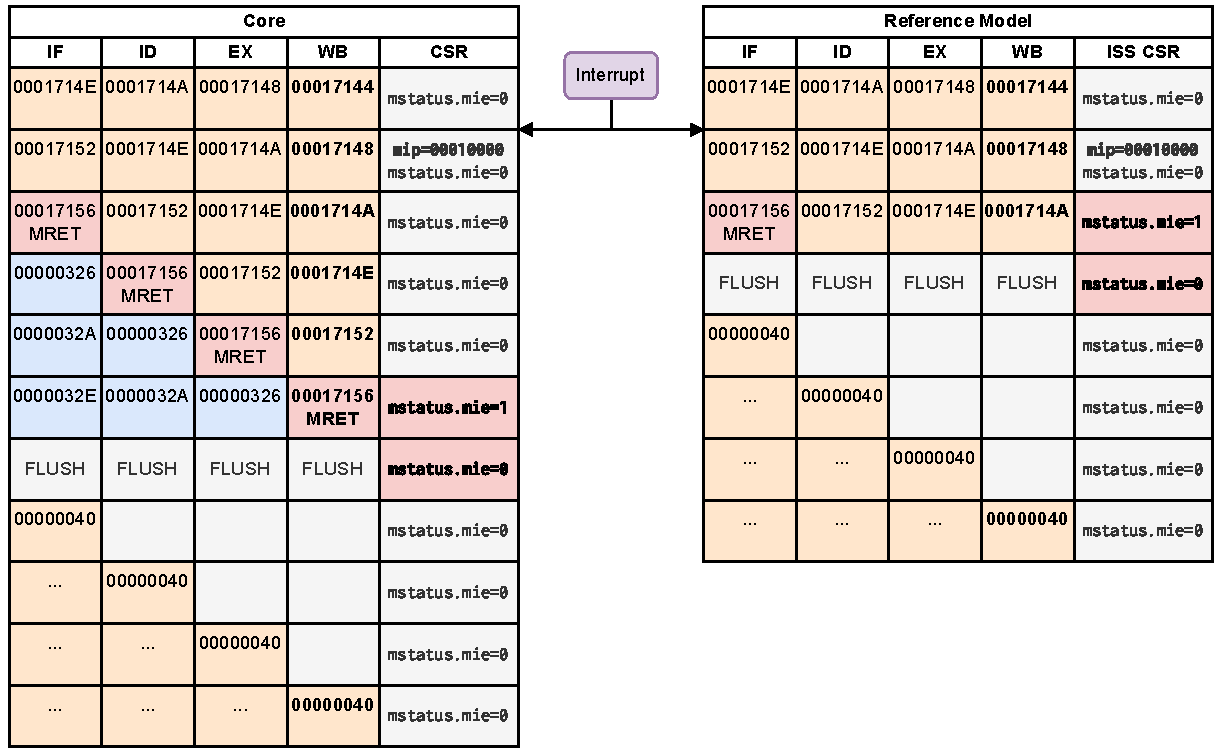
\includegraphics[width=1\linewidth]{figures/mret_example_fail.pdf}
    \caption{Example showing the mismatch of execution between the core and reference model when an interrupt is taken directly after another interrupt.}
    \label{fig:mret_example_fail}
\end{figure}


This can be highlighted with the example in \Cref{fig:mret_example_fail}. This shows the pipeline content of the core and reference model, aswell as the \rv{mie} bit in the \rv{mstatus} CSR. In the example, the reference model uses the CSR stored in the ISS to determine if interrupts are enabled or disabled.

The example shows an interrupt being applied while another interrupt handler is running (orange instructions). As explained in \Cref{sec:bg_interrupts}, when an interrupt is taken, and the interrupt handler starts running. This disables the \rv{mstatus.mie} bit. At the end of the interrupt handler, the \rv{mret} instruction runs to return to normal execution, and enables \rv{mstatus.mie} again. 


The example shows that when the \rv{mret} instruction runs in the ISS, \rv{mstatue.mie} is immediately enabled. If another interrupt is enabled at this point, the ISS would then take the next interrupt directly after the mret, instead of returning to the normal execution flow (green instructions) like the core does. We see that this causes the instructions with PC \rv{0001714E, 00017152, and 00017156} to not be retired from the core before the interrupt is taken.


\subsection{External CSR}

We must consider the timing of the CSR writes through the pipeline to avoid this mistake.

One way to do this is to add an external CSR to the pipeline shell. This can hold the CSRs that affect the interrupt timing and can be updated based on the propagation of the pipeline.


When calling the interrupt function in the ISS, we can add the updated contents of the external CSR to enable interrupts only when the CSR changes have properly propagated to the external CSR. This requires that the ISS takes these CSR values as inputs, giving us \Cref{issReq:set_CSR}.

CSR changes can be output with RVFI. Since the ISS's RVFI output already travels through the pipeline, we can use it to update the external CSR when the changes reach the WB stage. This requires the ISS to output these CSR changes through RVFI, giving us \Cref{issReq:CSR_out}.


\Cref{fig:mret_example} shows the same example as above, but the value from the external CSR is considered before taking an interrupt. The example shows both the CSR from the ISS and the external CSR.

\begin{figure}
    \centering
    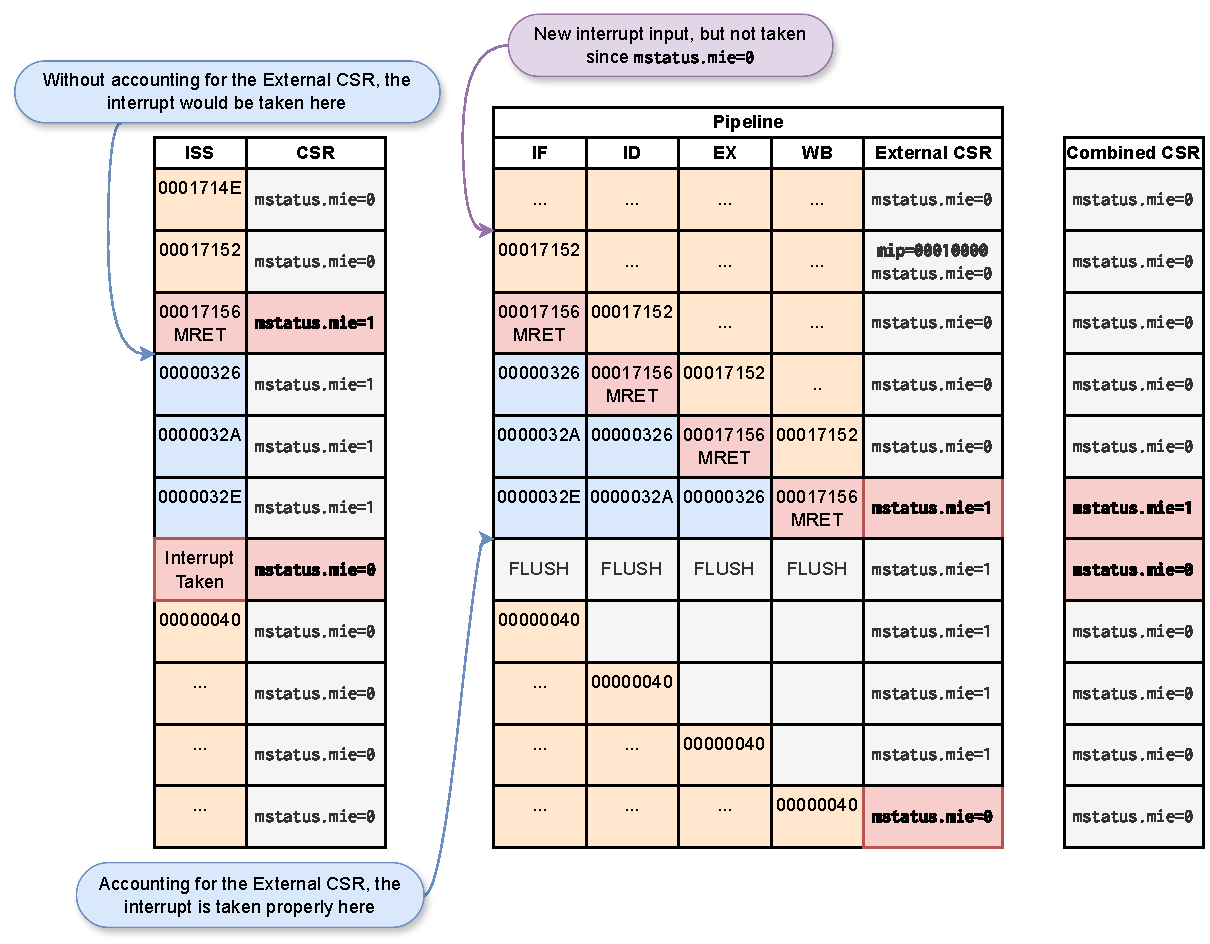
\includegraphics[width=1\linewidth]{figures/mret_example.pdf}
    \caption{Example showing how the timing of CSRs can influence interrupt timing.}
    \label{fig:mret_example}
\end{figure}

We see that in the ISS, the interrupt is not immediately taken after the \rv{mret} instruction, but instead taken when the external CSR changes to \rv{mstatus.mie=1}.

It can be beneficial to also use the CSR from the ISS, because although we want to delay the enabling of the interrupt, we want interrupts to be immediately disabled when an interrupt is taken. From the figure, we se the external CSR also delays the disabling of \rv{mstatus.mie}. If we only used the external CSR, new interrupts could be taken after another interrupt is taken. Because of this it is beneficial to use both the internal and external CSR.

The same problem can occur immediately following a write to the \rv{mie} CSR that enables a previously disabled \rv{irq}. It can also be solved the same way, by storing \rv{mie} in the external CSR.

\subsubsection{interrupt enabled}

CSRs are not always updated in the WB stage. \Cref{fig:interrupt_timing} shows the timing of interrupts in the core, and shows that the CSRs are updated one cycle after deciding to take the interrupt. Looking at \Cref{fig:mret_example}, we see that if we only wrote to the external CSR in the WB stage, interrupts would be enabled for 4 cycles after taking the interrupt.  

Therefore, the \sv{interrupt_enabled} signal sent to the ISS with \sv{iss_intr()} should go high when the \rv{mstatus.mie} reaches WB, but go low immediately after an interrupt is taken. This behavior is in \Cref{fig:mstatus_mie}, which shows how the signal can be modeled using the \sv{wb_mstatus.mie} signal generated from the WB stage, and the \sv{interrupt_taken} from \sv{iss_intr()}.

\begin{figure}[hbt]
    \centering
    \begin{tikztimingtable}
      \sv{clk}                  & 10{2C} G \\ 
      \sv{wb_mstatus.mie}       & LL   2{2H} 7{2L} \\ 
      \sv{interrupt_taken}      & 5{2L}  2{2H} 3{2L} \\ 
      \sv{interrupt_enabled}    & LL 6{2H} 3{2L} \\
    \end{tikztimingtable}
    \caption{Timing of \sv{interrupt_enable} and \sv{mstatus.mie}}
    \label{fig:mstatus_mie}
\end{figure}

%\tmp{TODO: talk about \sv{interrupt_enabled}}
%S
%
%
%
%
%\tmp{TODO: Hvorfor lagre csr i pipeline shell og ikke i ISS}
%\tmp{Lettere å få til å funke med core-independent approach.}
%
%
%
%
%\tmp{TODO: Mstatus endres feil, og bør også sendes inn i Spike}
%
%\begin{terminal}
% mstatus 00001880 / 0000000000001880 | INTR 0000     0 / 0000     0 |
% mstatus 00001880 / 0000000000001880 | INTR 0000     0 / 0000     0 | RVFI | ADDI     | 00006148
% mstatus 00001880 / 0000000000001880 | INTR 0000     0 / 0000     0 | RVFI | ADDI     | 0000614a
% mstatus 00001880 / 0000000000001880 | INTR 0000     0 / 0000     0 |
% mstatus 00001880 / 0000000000001880 | INTR 0000     0 / 0000     0 | RVFI | CSRRW    | 0000614e
% mstatus 00001880 / 0000000000000088 | INTR 0000     0 / 0000     0 | RVFI | CSRRW    | 00006152
% mstatus 00001880 / 0000000000000088 | INTR 0000     0 / 0000     0 |
% mstatus 00001880 / 0000000000000088 | INTR 0000     0 / 0000     0 |
% mstatus 00000088 / 0000000000000088 | INTR 0000     0 / 0000     0 |
%MIP set to: 40a8d3ff
% mstatus 00001880 / 0000000000000088 | INTR 0000     0 / 0000     0 | RVFI | MRET     | 00006156
% mstatus 00001880 / 0000000000000088 | INTR 0000     0 / 0000     0 |
% mstatus 00001880 / 0000000000000088 | INTR 0000     0 / 0000     0 |
% mstatus 00001880 / 0000000000000088 | INTR 0000     0 / 0000     0 |
% mstatus 00001880 / 0000000000000088 | INTR 0000     0 / 0000     0 |
% mstatus 00001880 / 0000000000001880 | INTR 0000     0 / 0000     0 |
% mstatus 00001880 / 0000000000001880 | INTR 0000     0 / 0000     0 |
% mstatus 00001880 / 0000000000001880 | INTR 0000     0 / 0000     0 |
% mstatus 00001880 / 0000000000001880 | INTR 005d    11 / 0000     0 |
% mstatus 00001880 / 0000000000001880 | INTR 005d    11 / 005d    11 | RVFI | JAL      | 0000002c
% mstatus 00001880 / 0000000000001880 | INTR 005d    11 / 005d    11 |
% mstatus 00001880 / 0000000000001880 | INTR 0000     0 / 005d    11 |
% mstatus 00001880 / 0000000000001880 | INTR 0000     0 / 0000     0 | RVFI | CSRRW    | 000059fc
%\end{terminal}


\section{Flushing}


\subsection{Flush after interrupt}

When the interrupt is taken, the remaining instructions in the pipeline must be \glsdisp{flush}{flushed}. This requires that the instructions in the pipeline should be set to 0, and the \sv{valid} signal be set to \sv{0}. This can be done by adding signals \sv{if_flush, id_flush, ex_flush}, and \sv{wb_flush} to each pipeline stage to flush each stage.

Since we only take interrupts when the pipeline can safely be flushed, we can directly use the \sv{interrupt_taken} signal to flush all the pipeline stages, as shown below.

\begin{systemverilog}
    assign flush_pipeline = interrupt_taken || debug_taken_q;

    always_comb begin
        if_flush_o <= flush_pipeline;
        id_flush_o <= flush_pipeline;
        ex_flush_o <= flush_pipeline;
        wb_flush_o <= flush_pipeline;
    end
\end{systemverilog}

\subsection{Flush after jump/branch}

A normal pipeline also flushes when the core jumps or branches to a new PC \cite{pattersonComputerOrganizationDesign2021}. Since we call the ISS in the IF stage, and the ISS fully executes one instruction before the next, the ISS always executes the correct instruction after a branch or jump, and we do not get the same incorrect instructions as the the core in the pipeline that need to be flushed.


The CV32E40S core executes jumps in the ID stage, and branches in the EX stage \cite{openhwgroupPipelineDetailsCOREV2023}. This means that the core and reference model can have a mismatch in the IF and ID stages before a jump or branch is correctly taken in the core.

Looking at \Cref{fig:dependency-tree-cv32x}, we see that the state of the IF is not required for interrupt timing, and that the state of ID is only considered if it contains a \acrshort{clic} pointer. Since we for the time being only support \acrshort{clint} interrupts, we can ignore flushing the pipeline because of jumps and branches, but this assumption should be evaluated again when implementing \acrshort{clic} interrupts in future work.

\section{State Revertion}
\label{sec:ps_revertion}

In a normal pipeline, where the state changes are applied in the WB stage, flushing each pipeline stage is sufficient to discard the effects of the instruction \cite[Ch. 4]{pattersonComputerOrganizationDesign2021}.

This is not necessarily the case for our pipeline implementation. Since the ISS executes the whole instruction before inputting the results into the IF stage, all the instruction's state changes are already written back inside the ISS. Since the changes have already been applied, flushing the pipeline does not discard them. To also discard these changes in the ISS, we need a way to revert the state of the ISS to a previous state.

This is one of the major disadvantages of calling the ISS in the IF stage compared to calling the ISS in the WB stage.


This is in some ways comparable to the rollback approach used by some lock-step processors \cite{marquesLockVHeterogeneousFault2021, liDuckCoreFaultTolerantProcessor2021, nikiemaDesignLowComplexity2023} to \textit{rollback} the processor context of two synced cores if they diverge. \textcite{marquesLockVHeterogeneousFault2021} saves the state of the processor at various \glspl{checkpoint} along the execution, and if a fault is found, the state is reverted to the previous valid checkpoint.

We can use a similar approach to store the state of the ISS into \textit{snapthots} we can revert back to. Since an interrupt and flush can happen at any instruction, we should have a checkpoint between every instruction.


To properly revert the state of the ISS, we must be able to revert all possible external changes caused by executing an instruction. The most important registers are the 32 \acrfull{gpr} and the \acrfull{pc}, which are written to or read from at almost every instruction \cite{watermanRISCVInstructionSet2019}.

Some \acrfull{csr} are also changed because of instructions and must be stored. Many CSRs are likely to remain static like the \rv{mvendorid}, \rv{misa}, and \rv{marchid}, while others may change during execution like \rv{mstatus}, \rv{mie}, and \rv{mscratch} \cite{watermanRISCVInstructionSet2021}. We can therefore either only store some relevant CSRs or store all CSRs.

Additionally, since we use the ISS's internal memory simulation, we also need to revert potential memory writes that occurred for instructions that must be discarded.


\subsection{Store states in PS or ISS}

We can store these states inside the ISS or in the Pipeline shell. By outputting the snapshot and moving it through the pipeline, it would in theory be simple to input the state of the oldest instruction in the pipeline into the ISS, and revert back to it. This could also be more practical if a core-independent pipeline shell is chosen in \Cref{sec:ps_dependency}. In practice, it may not necessarily be that easy to convert the snapshot into SystemVerilog and have it contained enough to be sent through the pipeline easily. Another solution could be not to store the state as a snapshot, but only the state changes. This would require iterating through the pipeline stages in reverse, and reversing all the stored state changes.

We choose to store the snapshot inside the ISS. This keeps the state contained and allows the snapshot to be stored in a logical format to the ISS without converting it to and from SystemVerilog to be sent through the pipeline. In order to revert the state from outside the ISS, we must use a function where we can specify the number of states to revert. This gives us \textbf{\Cref{issReq:revertState}}, specifying that the ISS must be able to revert to a previous state, reverting registers, CSRs, and memory operations.

\subsection{When to revert}

The order of events when reverting the state is important to get right.
The naive order could look something like this:

\begin{enumerate}
    \item Interrupt input into RM
    \item RM decides interrupt is allowed and inputs the \rv{irq} bits into ISS to set the \rv{mip}.
    \item The ISS reports that the interrupt will be taken
    \item The pipeline shell is flushed
    \item The ISS reverts to a previous state
    \item The ISS starts running the interrupt handler
\end{enumerate}

This order is problematic. When the we run the \sv{iss_intr()} function and the interrupt is taken in the ISS, this sets the \rv{mepc} and \rv{mstatus} CSRs as explained in \Cref{sec:bg_interrupts}. By reverting the state after the interrupt is taken in the ISS like above, this discards these CSR writes, since the CSRs are reverted to a previous state. Since interrupt taking is decided inside the ISS, we can also not revert the state before running the \sv{iss_intr()} function.

We must therefore revert the state before setting the \rv{mip}, but after deciding that the interrupt will be taken. We choose to revert the state from inside the ISS, instead of using a separate \sv{iss_revert()} function from the pipeline shell. We therefore add a \sv{revert_steps} parameter to the \sv{iss_revert()} function, so state revertion can be done inside the ISS.

This gives us the following order:

\begin{enumerate}
    \item Interrupt input into RM
    \item The RM decides if interrupts are allowed and inputs \
    Determine if interrupt will be taken with the incoming interrupt
    \item RM decides interrupt is allowed and inputs the \rv{irq} bits into ISS to set the \rv{mip}.
    \item - The ISS decides the interrupt will be taken
    \item - The ISS reverts the state
    \item - The ISS takes the interrupt and writes to the relevant CSRs
    \item The pipeline shell is flushed
    \item The ISS starts running the interrupt handler and 
\end{enumerate}

\subsection{How many states to revert}

To determine the amount of steps to revert, we can use the example in \Cref{fig:revert_example}.
This shows the PC of the instructions in the pipeline shell, and the PC of instructions executed in the ISS. In the WB stage, we see the retired instructions in bold, which are output over RVFI. The reference model decides that interrutps are allowed after \sv{1504} is retired and calls \sv{iss_intr()}. Since \sv{1504} is the last instruction to retire, we need to discard the changes from \sv{150a}, \sv{1508}, and \sv{1506} by reverting the state of the ISS to the state before it executed \sv{1506}. After the revertion is done, the ISS can take the interrupt, and \sv{1506} will be stored in the \rv{mepc} CSR and be the first instruction to run when the interrupt handler is completed.

With the current implementation, we see that we always need to revert the same number of instructions for a given pipeline depth. In the case of the CV32E40S with 4 pipeline stages, we need to revert 3 instructions.

\begin{figure}
    \centering
    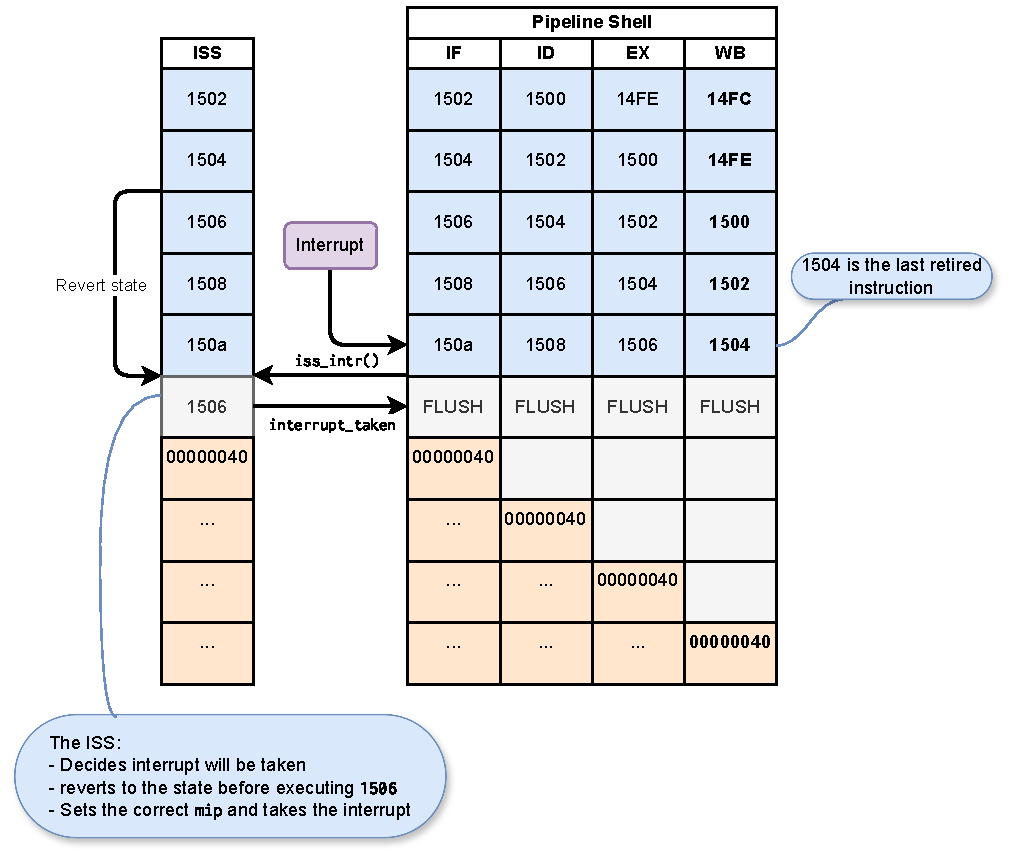
\includegraphics[width=0.85\linewidth]{figures/revert_example.pdf}
    \caption{Example showing the how many instructions we need to revert the state by, when flushing the pipeline.}
    \label{fig:revert_example}
\end{figure}


%
%\begin{figure}[htb]
%\centering
%\begin{ganttchart}[
		x unit=1.4cm,
		y unit chart=0.7cm,
		canvas/.style={draw=none,fill=none}, % remove canvas borders, etc
		vgrid={*{2}{draw=black!8}},           % vertical gray lines every unit
		inline,                              % draw bars inline
		group/.style={draw=none,fill=none},  % remove group borders, etc
		bar top shift=0.1,                   % give bar 10% padding top/bottom
		bar height=0.8,                      % bar size 80% of vertical space
		y unit title=0.5cm,                  % crop titles a little smaller
		title/.style={draw=none,fill=none},  % remove title borders, etc
		include title in canvas=false        % no vertical grid in title
	]{-2}{4}

    %\gantttitlelist{Cycle,IF,ID,EX,WB}{1}

	\gantttitle{Cycle}{-1}
	\gantttitle{ISS}{3}
 
	\gantttitle{}{1}
	\gantttitle{IF}{-1}
	\gantttitle{ID}{3}
	\gantttitle{EX}{-1}
	\gantttitle{WB}{3} \\

	\ganttgroup[inline=false]{1}{0}{4}
	\ganttbar[bar/.style={draw=black!80,fill=orange!40},name=iss0 ]{1}{-2}{-2}
	\ganttbar[bar/.style={draw=black!80,fill=orange!40}  ]{1}{0}{0}\\
 
	\ganttgroup[inline=false]{2}{0}{4}
	\ganttbar[bar/.style={draw=black!80,fill=yellow!40}, name=iss1  ]{2}{-2}{-2}
	\ganttbar[bar/.style={draw=black!80,fill=yellow!40}  ]{2}{0}{0}
	\ganttbar[bar/.style={draw=black!80,fill=orange!40}  ]{1}{1}{1}\\
 
	\ganttgroup[inline=false]{3}{0}{4}
	\ganttbar[bar/.style={draw=black!80,fill=lime!40},name=iss2    ]{3}{-2}{-2}
	\ganttbar[bar/.style={draw=black!80,fill=lime!40}    ]{3}{0}{0}
	\ganttbar[bar/.style={draw=black!80,fill=yellow!40}  ]{2}{1}{1}
	\ganttbar[bar/.style={draw=black!80,fill=orange!40}  ]{1}{2}{2}\\
 
	\ganttgroup[inline=false]{4}{0}{4}
	\ganttbar[bar/.style={draw=black!80,fill=green!40},name=iss3   ]{4}{-2}{-2}
	\ganttbar[bar/.style={draw=black!80,fill=green!40}   ]{4}{0}{0}
	\ganttbar[bar/.style={draw=black!80,fill=lime!40}    ]{3}{1}{1} 
	\ganttbar[bar/.style={draw=black!80,fill=yellow!40}  ]{2}{2}{2} 
	\ganttbar[bar/.style={draw=black!80,fill=orange!40}  ]{1}{3}{3} 
	\ganttbar[bar/.style={draw=none}  ]{\textbf{valid}}{4}{4} \\
 
	\ganttgroup[inline=false]{(IRQ) 5}{0}{4}
    \ganttbar[bar/.style={draw=black!80,fill=cyan!40},name=iss4    ]{5}{-2}{-2} 
    \ganttbar[bar/.style={draw=black!80,fill=cyan!40}    ]{5}{0}{0} 
	\ganttbar[bar/.style={draw=black!80,fill=green!40}   ]{4}{1}{1}
	\ganttbar[bar/.style={draw=black!80,fill=lime!40}    ]{3}{2}{2} 
	\ganttbar[bar/.style={draw=black!80,fill=yellow!40}  ]{2}{3}{3}  
	\ganttbar[bar/.style={draw=none}  ]{\textbf{valid}}{4}{4} \\


	\ganttgroup[inline=false]{(Revert(2)) 6}{0}{1}
    \ganttbar[bar/.style={draw=black!80,fill=black!10},name=iss5    ]{3}{-2}{-2} 
    \ganttbar[bar/.style={draw=black!80,fill=black!10}    ]{}{0}{0} 
    \ganttbar[bar/.style={draw=black!80,fill=black!10}    ]{}{1}{1} 
    \ganttbar[bar/.style={draw=black!80,fill=black!10}    ]{}{2}{2} 
    \ganttbar[bar/.style={draw=black!80,fill=black!10}    ]{}{3}{3} 
    
    \\
    
	\ganttgroup[inline=false]{7}{0}{1}
	\ganttbar[bar/.style={draw=black!80,fill=red!50}]{IH1}{-2}{-2}
	\ganttbar[bar/.style={draw=black!80,fill=red!50}]{IH1}{0}{0} \\

	\ganttgroup[inline=false]{8}{0}{1}
	\ganttbar[bar/.style={draw=black!80,fill=orange!80}    ]{IH2}{-2}{-2}
	\ganttbar[bar/.style={draw=black!80,fill=orange!80}    ]{IH2}{0}{0}
	\ganttbar[bar/.style={draw=black!80,fill=red!50}       ]{IH1}{1}{1} \\
	
	\ganttgroup[inline=false]{9}{0}{1}
	\ganttbar[bar/.style={draw=black!80,fill=yellow!80}    ]{IH3}{-2}{-2}
	\ganttbar[bar/.style={draw=black!80,fill=yellow!80}    ]{IH3}{0}{0}
	\ganttbar[bar/.style={draw=black!80,fill=orange!80}    ]{IH2}{1}{1}
	\ganttbar[bar/.style={draw=black!80,fill=red!50}       ]{IH1}{2}{2} \\
 
	\ganttgroup[inline=false]{10}{0}{1}
	\ganttbar[bar/.style={draw=black!80,fill=lime}       ]{IH4}{-2}{-2}
	\ganttbar[bar/.style={draw=black!80,fill=lime}       ]{IH4}{0}{0}
	\ganttbar[bar/.style={draw=black!80,fill=yellow!80}    ]{IH3}{1}{1}
	\ganttbar[bar/.style={draw=black!80,fill=orange!80}    ]{IH2}{2}{2}
	\ganttbar[bar/.style={draw=black!80,fill=red!50}       ]{IH1}{3}{3}  
	\ganttbar[bar/.style={draw=none}  ]{\textbf{valid}}{4}{4}\\


    \ganttlink[]{iss2}{iss5}

    %\ganttlink[link type=rdldr]{[xshift=-0.3cm]iss3.east}{[yshift=1cm]iss3.east}{[yshift=1cm]iss2.east}
    %\ganttlink[]{[yshift=1cm]iss4.east}{[yshift=1cm]iss3.east}

\end{ganttchart}

%\caption{\tmp{TODO: fix figure}Illustrate state reversion with ISS content and pipeline content.}
%\label{fig:interrupt_revert_addi}
%\end{figure}
%
%\begin{figure}[htb]
%\centering
%\begin{ganttchart}[
		x unit=1.4cm,
		y unit chart=0.7cm,
		canvas/.style={draw=none,fill=none}, % remove canvas borders, etc
		vgrid={*{2}{draw=black!8}},           % vertical gray lines every unit
		inline,                              % draw bars inline
		group/.style={draw=none,fill=none},  % remove group borders, etc
		bar top shift=0.1,                   % give bar 10% padding top/bottom
		bar height=0.8,                      % bar size 80% of vertical space
		y unit title=0.5cm,                  % crop titles a little smaller
		title/.style={draw=none,fill=none},  % remove title borders, etc
		include title in canvas=false        % no vertical grid in title
	]{-2}{4}

    %\gantttitlelist{Cycle,IF,ID,EX,WB}{1}

	\gantttitle{Cycle}{-1}
	\gantttitle{ISS}{3}
 
	\gantttitle{}{1}
	\gantttitle{IF}{-1}
	\gantttitle{ID}{3}
	\gantttitle{EX}{-1}
	\gantttitle{WB}{3} \\

	\ganttgroup[inline=false]{1}{0}{4}
	\ganttbar[bar/.style={draw=black!80,fill=orange!40},name=iss0 ]{1}{-2}{-2}
	\ganttbar[bar/.style={draw=black!80,fill=orange!40}  ]{1}{0}{0}\\
 
	\ganttgroup[inline=false]{2}{0}{4}
	\ganttbar[bar/.style={draw=black!80,fill=yellow!40}, name=iss1  ]{2}{-2}{-2}
	\ganttbar[bar/.style={draw=black!80,fill=yellow!40}  ]{2}{0}{0}
	\ganttbar[bar/.style={draw=black!80,fill=orange!40}  ]{1}{1}{1}\\
 
	\ganttgroup[inline=false]{3}{0}{4}
	\ganttbar[bar/.style={draw=black!80,fill=lime!40},name=iss2    ]{3}{-2}{-2}
	\ganttbar[bar/.style={draw=black!80,fill=lime!40}    ]{3}{0}{0}
	\ganttbar[bar/.style={draw=black!80,fill=yellow!40}  ]{2}{1}{1}
	\ganttbar[bar/.style={draw=black!80,fill=orange!40}  ]{1}{2}{2}\\
 
	\ganttgroup[inline=false]{4}{0}{4}
	\ganttbar[bar/.style={draw=black!80,fill=green!40},name=iss3   ]{4}{-2}{-2}
	\ganttbar[bar/.style={draw=black!80,fill=green!40}   ]{4}{0}{0}
	\ganttbar[bar/.style={draw=black!80,fill=lime!40}    ]{3}{1}{1} 
	\ganttbar[bar/.style={draw=black!80,fill=yellow!40}  ]{2}{2}{2} 
	\ganttbar[bar/.style={draw=black!80,fill=orange!40}  ]{1}{3}{3} 
	\ganttbar[bar/.style={draw=none}  ]{\textbf{valid}}{4}{4} \\
 
	\ganttgroup[inline=false]{5}{0}{4}
    \ganttbar[bar/.style={draw=black!80,fill=cyan!40},name=iss4    ]{5}{-2}{-2} 
    \ganttbar[bar/.style={draw=black!80,fill=cyan!40}    ]{5}{0}{0} 
	\ganttbar[bar/.style={draw=black!80,fill=green!40}   ]{4}{1}{1}
	\ganttbar[bar/.style={draw=black!80,fill=lime!40}    ]{3}{2}{2} 
	\ganttbar[bar/.style={draw=black!80,fill=yellow!40}  ]{2}{3}{3}  
	\ganttbar[bar/.style={draw=none}  ]{\textbf{valid}}{4}{4} \\

	\ganttgroup[inline=false]{6}{0}{4}
    \ganttbar[bar/.style={draw=black!80,fill=cyan!40}    ]{5}{0}{0} 
	\ganttbar[bar/.style={draw=black!80,fill=green!40}   ]{4}{1}{1}
	\ganttbar[bar/.style={draw=black!80,fill=lime!40}    ]{3}{2}{2} 
	\ganttbar[bar/.style={draw=black!80,fill=yellow!40}  ]{2}{3}{3}  
	   \\

	\ganttgroup[inline=false]{(IRQ) 7}{0}{4}
    \ganttbar[bar/.style={draw=black!80,fill=cyan!40}    ]{5}{0}{0} 
	\ganttbar[bar/.style={draw=black!80,fill=green!40}   ]{4}{1}{1}
	\ganttbar[bar/.style={draw=black!80,fill=lime!40}    ]{3}{2}{2} 
	\ganttbar[bar/.style={draw=black!80,fill=yellow!40}  ]{2}{3}{3}  
	\\



	\ganttgroup[inline=false]{(Revert(3)) 8}{0}{1}
    \ganttbar[bar/.style={draw=black!80,fill=black!10},name=issRev    ]{3}{-2}{-2} 
    \ganttbar[bar/.style={draw=black!80,fill=black!10}    ]{}{0}{0} 
    \ganttbar[bar/.style={draw=black!80,fill=black!10}    ]{}{1}{1} 
    \ganttbar[bar/.style={draw=black!80,fill=black!10}    ]{}{2}{2} 
    \ganttbar[bar/.style={draw=black!80,fill=black!10}    ]{}{3}{3} 
    
    \\
    
	\ganttgroup[inline=false]{9}{0}{1}
	\ganttbar[bar/.style={draw=black!80,fill=red!50}]{IH1}{-2}{-2}
	\ganttbar[bar/.style={draw=black!80,fill=red!50}]{IH1}{0}{0} \\

	\ganttgroup[inline=false]{10}{0}{1}
	\ganttbar[bar/.style={draw=black!80,fill=orange!80}    ]{IH2}{-2}{-2}
	\ganttbar[bar/.style={draw=black!80,fill=orange!80}    ]{IH2}{0}{0}
	\ganttbar[bar/.style={draw=black!80,fill=red!50}       ]{IH1}{1}{1} \\
	
	\ganttgroup[inline=false]{11}{0}{1}
	\ganttbar[bar/.style={draw=black!80,fill=yellow!80}    ]{IH3}{-2}{-2}
	\ganttbar[bar/.style={draw=black!80,fill=yellow!80}    ]{IH3}{0}{0}
	\ganttbar[bar/.style={draw=black!80,fill=orange!80}    ]{IH2}{1}{1}
	\ganttbar[bar/.style={draw=black!80,fill=red!50}       ]{IH1}{2}{2} \\
 
	\ganttgroup[inline=false]{12}{0}{1}
	\ganttbar[bar/.style={draw=black!80,fill=lime}       ]{IH4}{-2}{-2}
	\ganttbar[bar/.style={draw=black!80,fill=lime}       ]{IH4}{0}{0}
	\ganttbar[bar/.style={draw=black!80,fill=yellow!80}    ]{IH3}{1}{1}
	\ganttbar[bar/.style={draw=black!80,fill=orange!80}    ]{IH2}{2}{2}
	\ganttbar[bar/.style={draw=black!80,fill=red!50}       ]{IH1}{3}{3}  
	\ganttbar[bar/.style={draw=none}  ]{\textbf{valid}}{4}{4}\\


    \ganttlink[]{iss2}{issRev}

    %\ganttlink[link type=rdldr]{[xshift=-0.3cm]iss3.east}{[yshift=1cm]iss3.east}{[yshift=1cm]iss2.east}
    %\ganttlink[]{[yshift=1cm]iss4.east}{[yshift=1cm]iss3.east}

\end{ganttchart}

%\caption{\tmp{TODO: fix figure} Illustrate state reversion with ISS content and pipeline content.}
%\label{fig:interrupt_revert_divu}
%\end{figure}






\section{Other asynchronous events : \Cref{psReq:async_control}}
\tmp{TODO: Rydd opp litt}

As the previous sections used interrupts as an example of how asynchronous events are handled, this section will cover how the work done with interrupts transfers to other asynchronous events like debug requests and \acrfull{nmi}.
We will also cover some of the extra complexity that occurs when different types of asynchronous events appear simultaneously.

\subsection{Debug requests and similarities to interrupts}

We will use debug requests as an example of how other asynchronous events can utilize the techniques discovered for interrupts.


CV32E40S supports the debug specification from \cite{pauldonahueRISCVDebugSupport2023} \cite{openhwgroupDebugTriggerCOREV2023}.

\sv{debug_req_i} is used to externally trigger a debug event and can be thought of as the "debug interrupt" \cite{openhwgroupDebugTriggerCOREV2023}.


\subsection{Similarities to interrutps}

Multiple special cases from interrupts are transferable to debug requests. Some of these cases will be covered below.

\subsubsection{Informing the ISS of debug requests}


We can inform the ISS of debug requests the same way is interrupts in \Cref{sec:ps_interrupt}, by using a \sv{iss_set_debug(...)} function.

In the core, taking debug requests is determined similarly to interrupts by using the signals \sv{pending_async_debug} and \sv{async_debug_allowed}. We can partition these the same way as interrupts, where the ISS decides if the debug request is taken using inputs from the pipeline shell.

\subsubsection{Revertion after debug}

When an external debug request is taken, we need to change the PC to the debug handler. Like when interrupts are take, this also requires that the pipeline is flushed. This gives the same problem as interrupts in \Cref{sec:ps_revertion}, where the ISS needs to be reverted to a previous state. This can be implemented the same way as for interrupts, where the \sv{iss_set_debug()} function takes in the number of states to revert, and reverts the state if the debug request is taken. 

\subsubsection{Delay debug mode with pipeline}

The debug mode of the processor causes a similar problem to \rv{mstatus.mie} explained in \Cref{sec:ps_side-effects}, where the value changes too early in the ISS, and needs to be delayed with an external CSR. This can for example be a problem when a debug handler returns and immediately goes straight into another debug request. This is similar to the example with \rv{mret} in \Cref{fig:mret_example_fail}. To solve this, we also propagate the debug mode signal through the pipeline, considering this before taking debug requests and interrupts.


%\subsubsection{Two debug requests after each other}
%
%We get the same problem when a debug request returns from debug mode with \rv{dret} and goes straight into another debug request, as when an interrupt returns from the interrupt handler with \rv{mret} and takes another interrupt. The problem here is that the ISS runs a few instructions ahead and applies the side effects of the \rv{dret} instruction prematurely, causing the \sv{iss_set_debug()} function to set \sv{debug_taken} and flush the pipeline prematurely.
%
%This is solved for interrupts by exporting the relevant CSRs through RVFI, passing them through the pipeline to an external CSR, and using these to correctly time the changes.
%
%\rv{dret} restores the PC and privileged to the values stored in \rv{dpc} and \rv{dcsr}, and exits debug mode. The side effect that influences the timing of debug requests is that \ccode{debug_mode} is turned off in \rv{dret}. the \ccode{debug_mode} is used by the \ccode{set_debug} method to determine if a new debug request can be made, or if the processor is currently in the debug mode. We must therefore delay this signal to when the pipeline shell is out of debug mode, and not only when spike has exited debug mode. 
%
%The debug mode is output to RVFI via the \sv{rvfi_dbg_mode} signal. One solution is therefore to use this to update a copy of \sv{debug_mode} in the pipeline shell. One problem with this is that the \sv{rvfi_dbg_mode} reports high when in \rv{dret} since the instruction is run in debug mode, but since \rv{dret} disables debug mode, we want to set our local copy to 0 when the \rv{dret} instruction leaves WB. 
%
%\tmp{TODO: solve this. Pass a separate dbg mode signal through the stages, update internally in spike with saved states, or have a special "if dret" signal to set debug mode to 0}
%
%\subsection{debug at the very start}
%
%\tmp{Debug asserted from the beginning causes problems with state revertion, since it tries to revert more instructions than are stored in the previous states.}



\subsection{interrupts and debug at the same time}

When both interrupts and debug requests can happen at the same time, this can also lead to more problems. One example is when we return from debug mode and immediately take an interrupt. The delayed values of the debug mode can also affect interrupt timings. 
When considering multiple asynchronous events, we can not separate handling of interrupts and debug requests since these affect each other.

%For this to function correctly must disable the debug mode register in the external CSR, instantly, the same way as mret must ins \ref{}

%In the example, the ISS takes the interrupt immediately after executing mret in IF, before the debug mode change from dret has propagated to WB. 
%
%-> interrupt allowed signal in spike not used correctly
%
%The privileged level overwrites \ccode{m_enabled}. Privelegde was lower than M(3). WHy?? did dcsr store the wrong privilege \tmp{TODO}
%
%\begin{table}
%    \centering
%    \begin{tabular}{cc}
%        addi & addi\\
%        wfi & wfi\\
%        dret & dret\\
%        mret & \\
%         & \\
%         & \\
%         & \\
%    \end{tabular}
%    \caption{Caption}
%    \label{tab:my_label}
%\end{table}
%\begin{terminal}
%addi            
%wfi             
%dret
%mret
%-INTR11 - jal
%
%\end{terminal}


\subsection{priorotizing events}

We also have to prioritize the events in relation to each other. Since we currently use the ISS to determine which asynchronous event to take, this must also take into account the prioritization between the different events. The prioritized list of the CV32E40S \cite{openhwgroupCv32e40s2024} is shown below.

\begin{enumerate}
    \item nmi
    \item async debug
    \item interrupt
    \item sync debug
    \item normal execution
    %\begin{enumerate}
    %    \item exception
    %    \item wfi
    %    \item fencei
    %    \item dret
    %    \item csr write
    %    \item csr flush
    %    \item branch
    %    \item jump
    %    \item clic ptr or meet ptr
    %\end{enumerate}
\end{enumerate}


%\subsection{CLIC Interrupts}
%
%CLIC and CLINT both use the same \sv{pending_interrupt} and \sv{interrupt_allowed} signals, but differ in how they take the interrupt.
%
%\subsection{NMI}
%
%\sv{pending_nmi} and \sv{nmi_allowed}.
%\sv{nmi_allowed} is equal to \sv{interrupt_allowed}, except \sv{!interrupt_blanking_q} is replaced by \sv{!(woke_to_debug_q || woke_to_interrupt_q)}
%
%
%
%
%
%
%\subsection{Similarities to CLINT interrupts}
%
%From above we see that \sv{lsu_interruptible_i}, \sv{fencei_ongoing clic_ptr_in_pipeline}, \sv{sequence_interruptible}, \sv{csr_flush_ack_q}, and \sv{ctrl_fsm_cs} are all common signals for \sv{interrupt_allowed}, \sv{async_debug_allowed}, and \sv{nmi_allowed}. These signals are the signals that are influenced by the pipeline contents, and solving how these can be used to properly time the asynchronous events is common for all of these events.
%
%
%By using CLINT interrupts as an example to verify if this approach for determining if an interrupt can be taken works, we can also assume that the same result will be applicable to CLIC interrupts, debug requests, and \acrshort{nmi}s by using \sv{async_debug_allowed}, \sv{nmi_allowed}, etc. 
%


%\subsection{WFI}
%
%\tmp{TODO}
%
%\tmp{We disable wfi in the ISS, so that the timing is done in the pipeline shell}

